\chapter{INFERENCE}

\renewcommand{\headrulewidth}{0.5pt}
\renewcommand{\footrulewidth}{0.5pt}
\thispagestyle{plain}
\pagestyle{fancy}
\fancyhf{}
\fancyhead[L]{\textbf{CHAPTER 3}}
\fancyhead[R]{\textbf{DROWSINESS DETECTION AND ALERT SYSTEM IN THE CAR}}
\raggedright
\fancyfoot[L]{From: Nguyen Van Anh Tuan}
\fancyfoot[R]{Page \thepage}

\section{Block Diagram}
    \begin{figure}[H]
        \centering
        
\includegraphics[width=0.6\linewidth]{img/block-diagram.png}
        \caption{Block diagram of system}
    \end{figure}
    \begin{figure}[H]
        \centering
        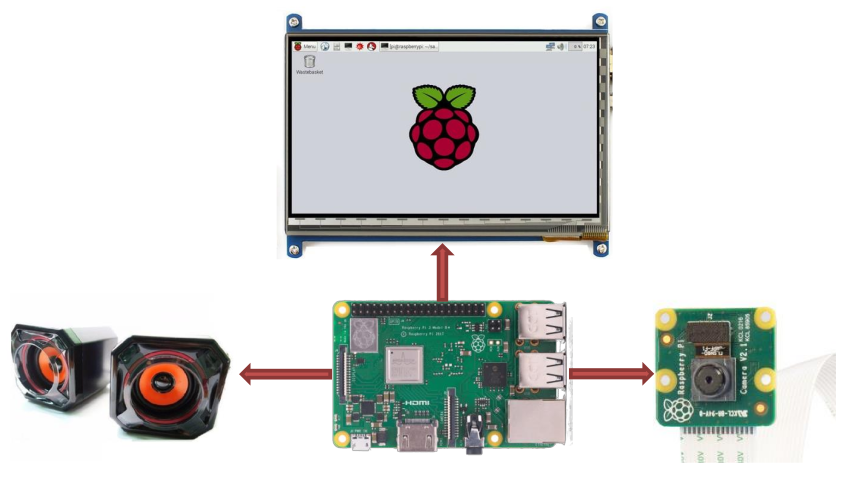
\includegraphics[width=0.6\linewidth]{img/Device-diagram.png}
        \caption{Device diagram of system}
    \end{figure}

\section{Flowchart}
    \begin{figure}[H]
        \centering
        \includegraphics[width=0.6\linewidth]{img/Flowchart.png}
        \caption{Flowchart of system}
    \end{figure}
    At first, we will set up a face-tracking camera to detect whether the driver is asleep or not (we are only interested in the eye area). 
    Extract eye area and calculate eye ratio to determine if eyes are closed or open, when it is determined that the eyes are closed, we 
    begin to count the number of frames that the eyes are closed, if the number of frames in which the eyes are closed exceeds the eye 
    threshold (parameters specified by the programmer), the person is considered to have dozed off and starts to issue an alarm.

    \subsection{Image From Camera}
    Initially, we will establish a connection with camera pi and take each image frame for processing, the input image will be an RGB image. 
    To access the ip camera, it is necessary to use the imutils library, which makes it easier to process images and work on OpenCV.
    \begin{figure}[H]
        \centering
        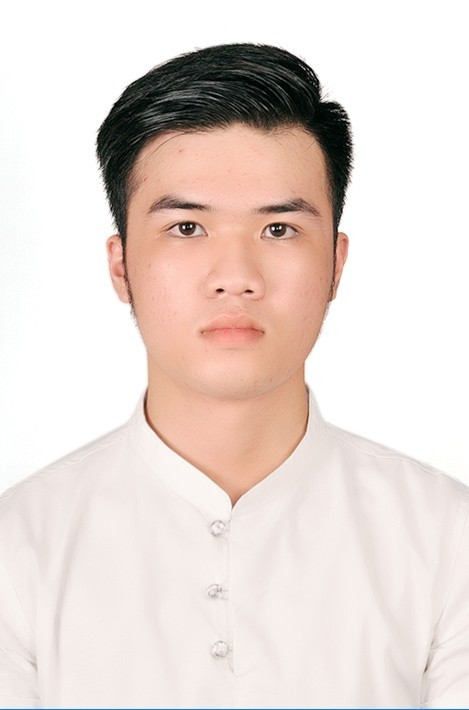
\includegraphics[width=0.6\linewidth]{img/1.JPG}
        \caption{Input image}
    \end{figure}

    \subsection{Pre-Processing}
        \begin{figure}[H]
            \centering
            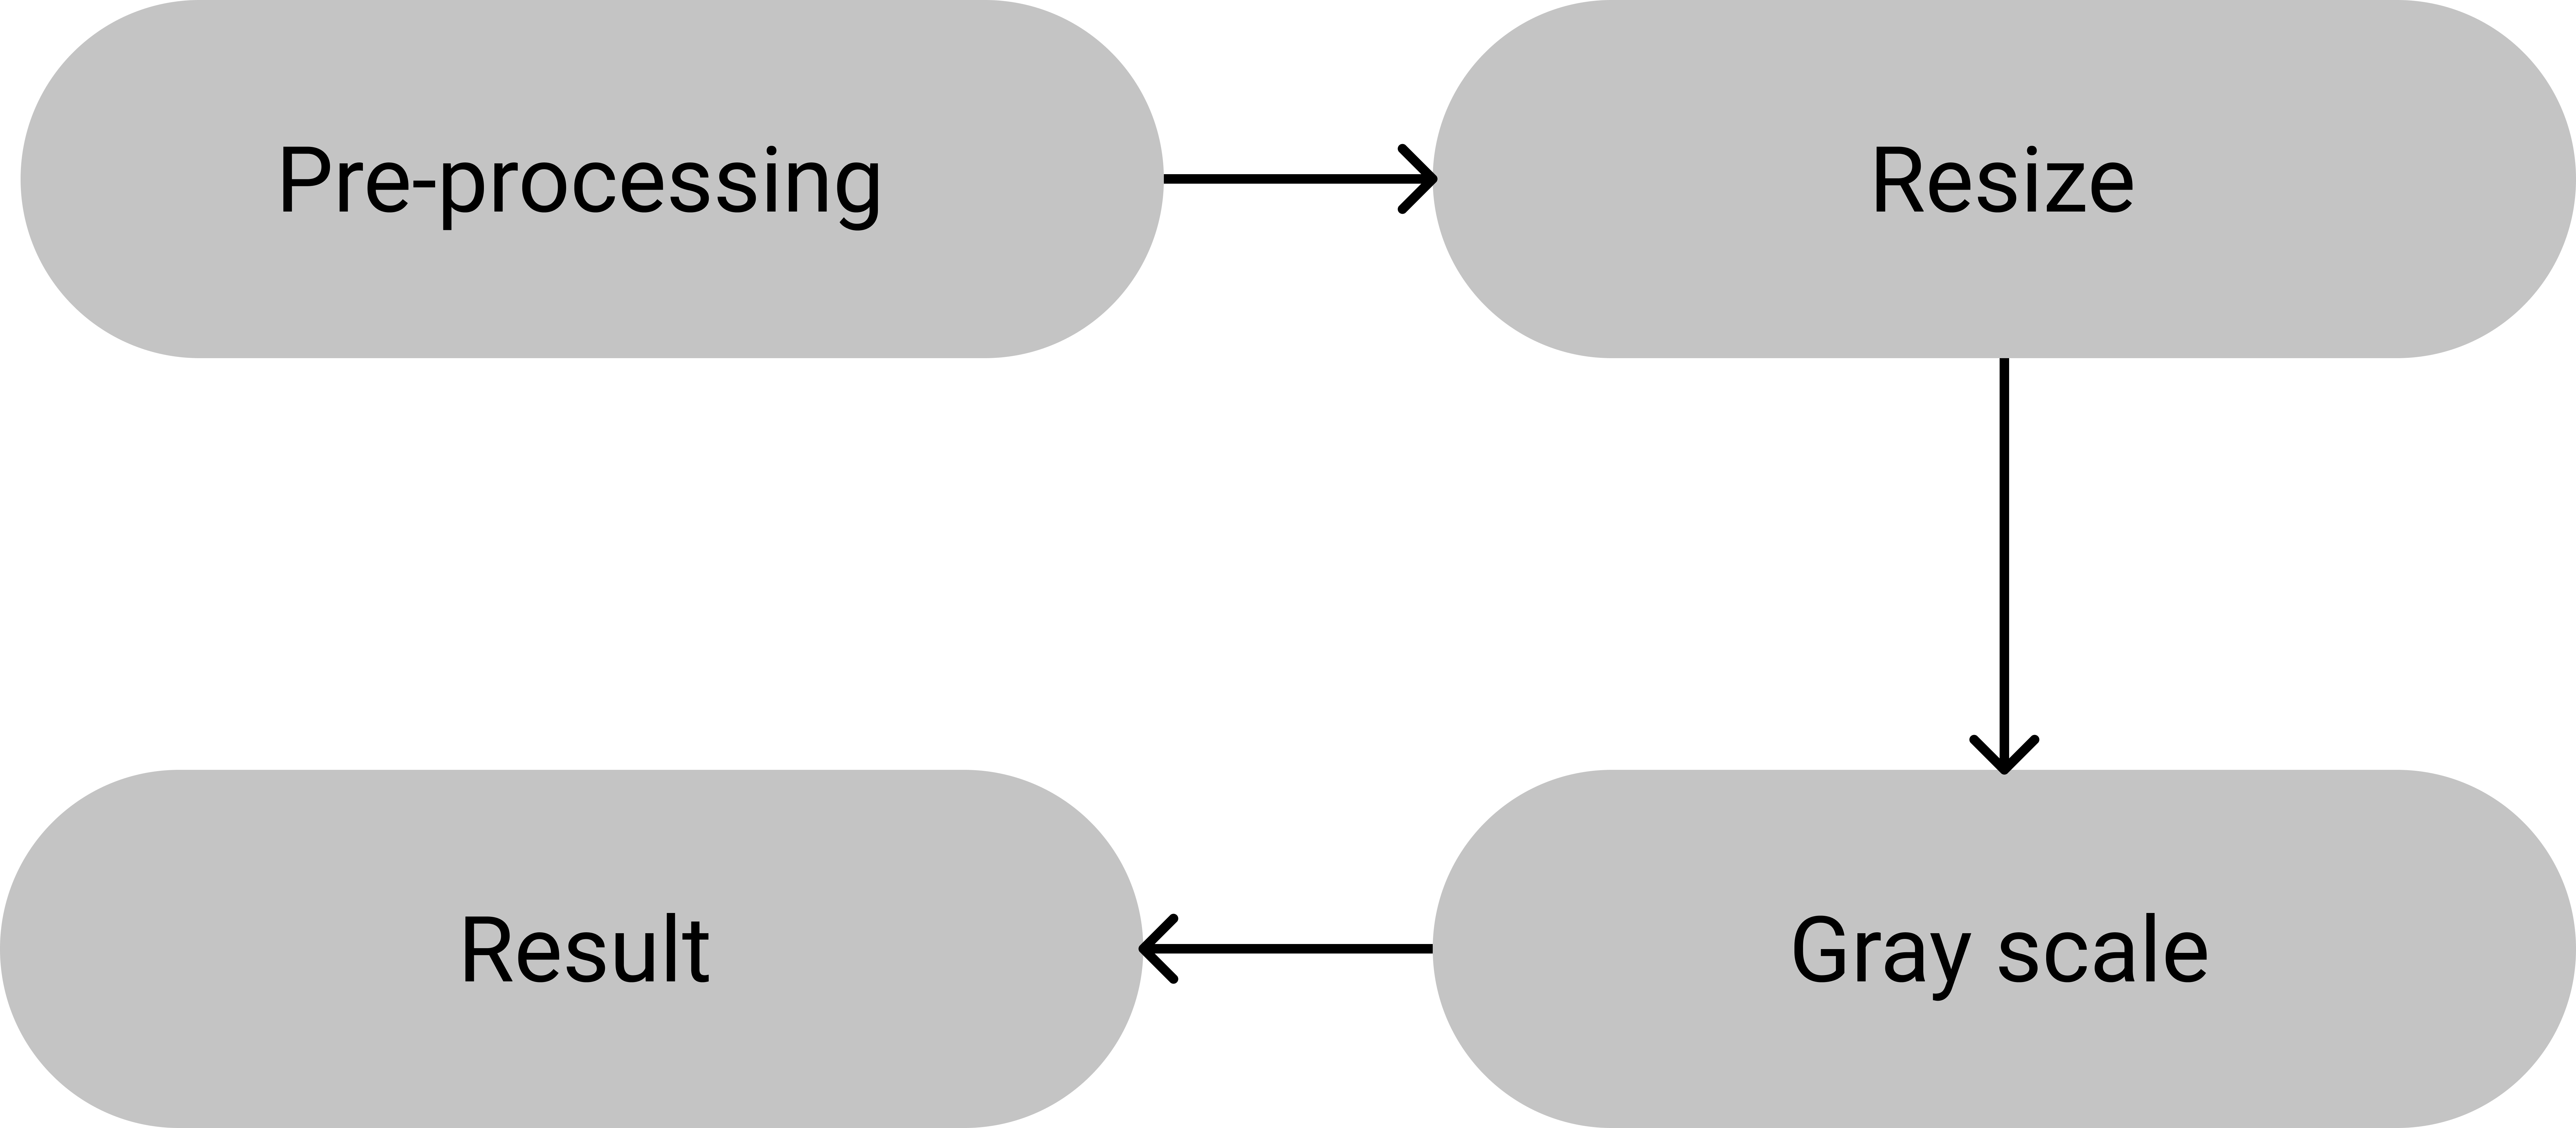
\includegraphics[width=0.6\linewidth]{img/pre-processing.png}
            \caption{Pre-processing}
        \end{figure}
        Start capturing images continously with infinite loops, then do pre-processing by resizing to get the desired width (450 pixels) and 
        convert it into gray-scale: $"gray=cv2.cvtColor(frame, cv2.COLOR\_BGR2GRAY)"$
        \begin{figure}[H]
            \centering
            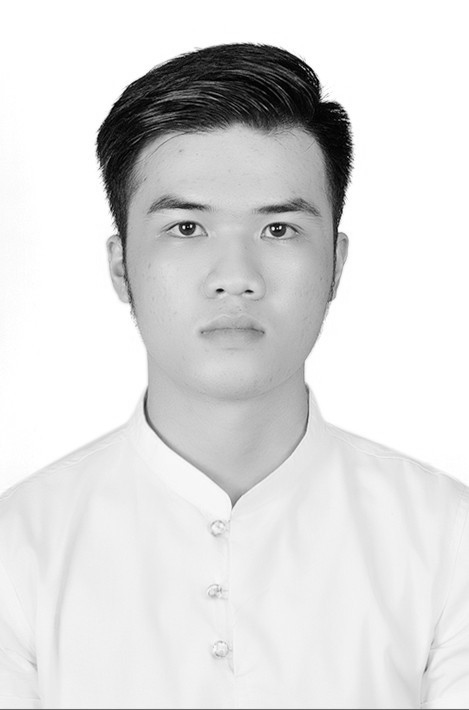
\includegraphics[width=0.6\linewidth]{img/Grayscale.png}
            \caption{Image after pre-processing}
        \end{figure}

    \subsection{Face Detection Using Haar-Like (Haar Cascade)}
        \begin{figure}[H]
            \centering
            
\includegraphics[width=0.6\linewidth]{img/Haar.png}
            \caption{Flowchart of face detection}
        \end{figure}
        To detect faces in an image, we need to convert the image to gray and then look at each single pixel and the points around it. Haar-Like 
        features are black and white rectangles segmented into different regions. It's basically using Haar type features and then using as many 
        of those features over many turns (cascade) to form a complete set of identifiers, and then proceed to draw recognizable faces on the 
        corner photo.
        \begin{figure}[H]
            \centering
            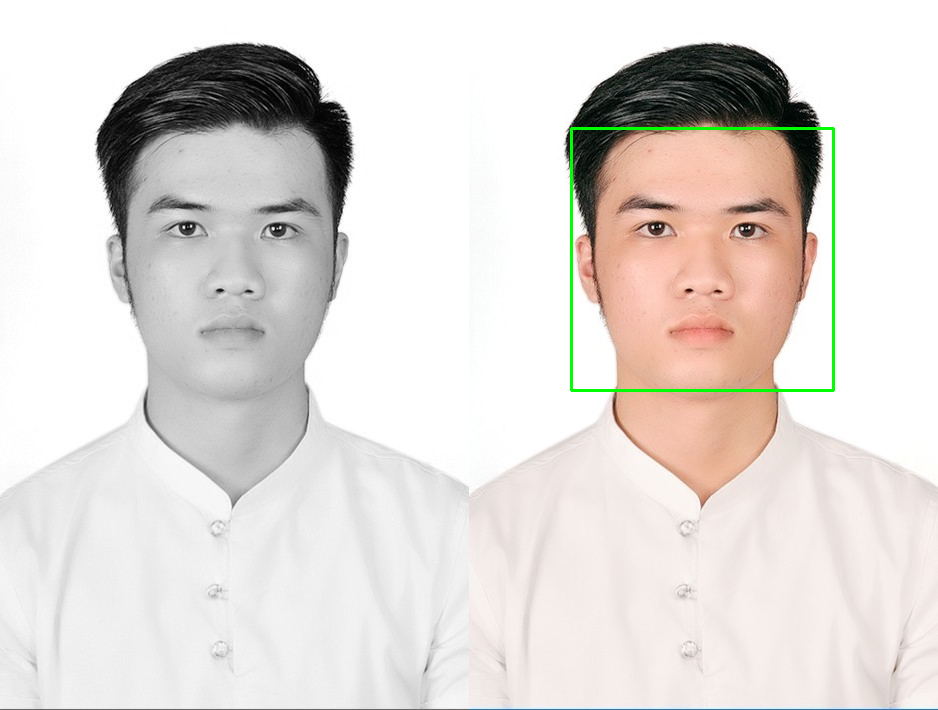
\includegraphics[width=0.6\linewidth]{img/Faces found.png}
            \caption{Face Detection}
        \end{figure}

    \subsection{Mark Facial Structure Using Facial Landmarks}
        \begin{figure}[H]
            \centering
            
\includegraphics[width=0.6\linewidth]{img/Figma.png}
            \caption{Facial landmarks}
        \end{figure}
        Using Dlib library's 68-point structure marking algorithm to locate facial parts including: eyes, nose, lip, eyebrows and face contour and 
        then mark all these points on image.
        \begin{figure}[H]
            \centering
            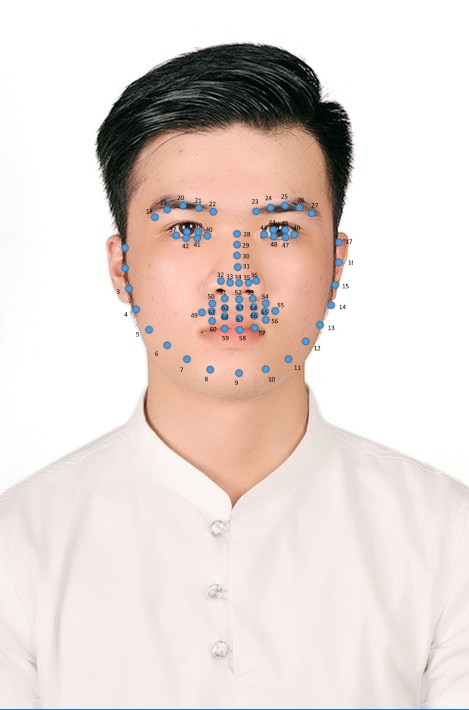
\includegraphics[width=0.6\linewidth]{img/testing.png}
            \caption{Mark 68 face points}
        \end{figure}

    \subsection{Extract The Eye Area}
        In this project, we just care about the eye area so we extract the eye area by using cut array Numpy, we can extract the coordinate (x,y) 
        of left eye and right eye.

    \subsection{Calculate Eye Ratio}
        With the extracted coordinate we will calculate the eye ratio, each eye is represented by 6 coordinates from $P_1$ to $P_6$.
        \begin{figure}[H]
            \centering
            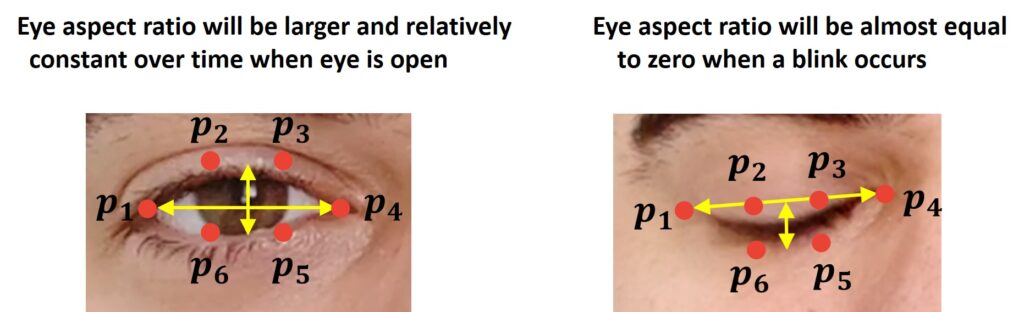
\includegraphics[width=0.6\linewidth]{img/eye-ratio.jpg}
            \caption{Extract eye ratio}
        \end{figure}
        There is a relationship between the width and height of these coordinates, we can use an equation that reflects this relationship called eye ratio (EAR).
        \begin{align}
            EAR = \frac{||P_2 - P_6|| + ||P_3 - P_5||}{2||P_1 - P_4||}
        \end{align}
        Which $P_1$ > $P_6$ are landmarks marked on the eyes, the numerator of this equation calculates the distance between the vertical landmarks 
        while the denominator calculates the distance between the horizontal landmarks. \\ 
        \vspace{3mm}
        The eye ratio is the distance that stays the same when the eyes are open, but rapidly decreases to zero when the eyes are closed or blinking. \\ 
        \vspace{3mm}
        By using this equation one can avoid complicated image processing techniques and simply rely on distance and time to determine whether the eyes are closed 
        or open. To make this more clear, consider the picture below from Soukupová and Čech:
        \begin{figure}[H]
            \centering
            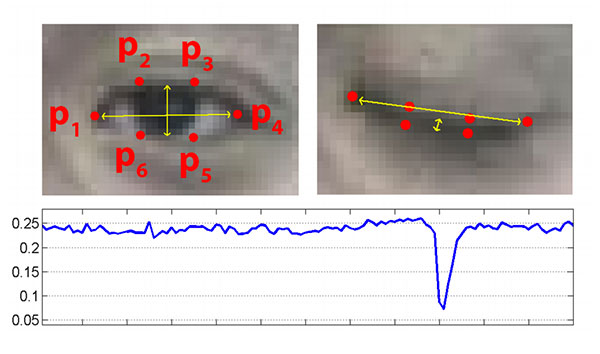
\includegraphics[width=0.6\linewidth]{img/calculate.png}
            \caption{Top-left: A visualization of eye landmarks when then the eye is open. Top-right: Eye landmarks when the eye is closed. Bottom: Plotting the eye aspect ratio over time.}
        \end{figure}

    \subsection{Drowsiness Detection}
        To detect sleep need to first set the program parameters: 
        \begin{itemize}
            \item Eye ratio threshold: to identify closed or open eyes. Determine the eye avg ratio by preparing 100 sample images including 50 
            eyes open and 50 closed eyes, examine each image to determine the threshold eye avg ratio, then average the eye avg ratio index to 
            select the threshold of eyes open and closed, based on information This number is used to compare and determine whether the eyes are 
            closed or open.
            \item Max sleep frames: to see if the person is awake or asleep
            \item $Alarmed = False$: initial state alarm is off 
        \end{itemize}

    \subsection{Alert}
        After determined that driver is asleep, we will turn on $"alarmed = True"$ to play a loudspeaker warning to wake the driver (using playsound library).
        \begin{figure}[H]
            \centering
            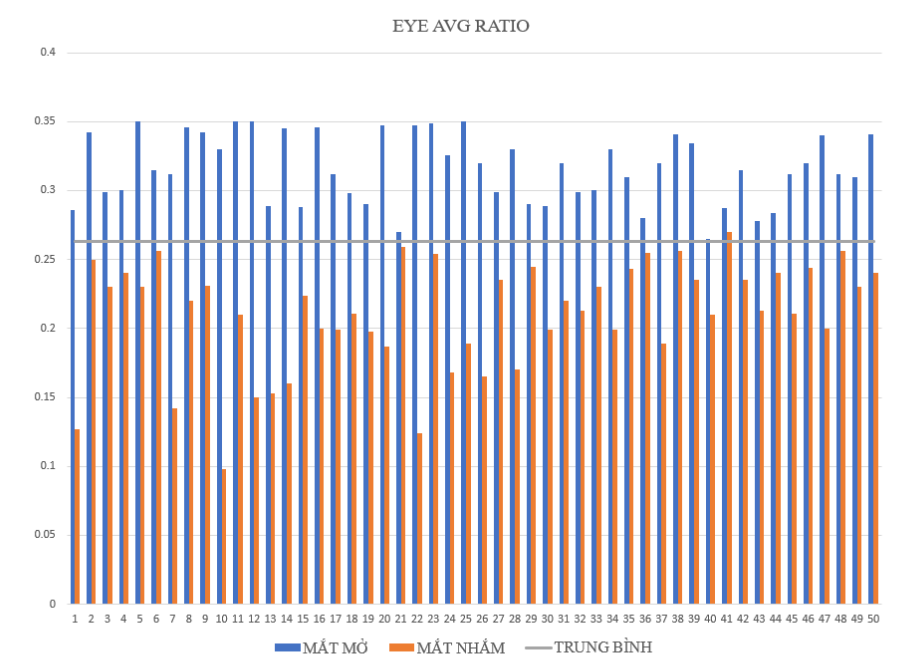
\includegraphics[width=0.6\linewidth]{img/eye-avg-ratio.png}
            \caption{Eye average ratio chart with 100 eye samples}
        \end{figure}